\documentclass[12pt,a4paper]{article}

% Idioma, codificacao e tipografia
\usepackage[T1]{fontenc}
\usepackage[utf8]{inputenc}
\usepackage[brazil]{babel}
\usepackage{newtxtext,newtxmath}
\usepackage{microtype}

% Formato da pagina segundo a apresentacao academica ABNT
\usepackage[a4paper,top=3cm,bottom=2cm,left=3cm,right=2cm,headheight=15pt,headsep=0.5cm]{geometry}
\usepackage{setspace}
\usepackage{ragged2e}
\usepackage{enumitem}
\usepackage{titlesec}
\usepackage{fancyhdr}
\usepackage[hidelinks]{hyperref}
\usepackage{xurl}
\usepackage{bookmark}
\usepackage{lastpage}
\usepackage{array}
\usepackage{booktabs}
\usepackage{longtable}
\usepackage{graphicx}
\usepackage{pdflscape}
\usepackage{caption}

\hypersetup{
  pdftitle={Sistema de Gestao de Drogaria},
  pdfsubject={Projeto de Banco de Dados},
  pdfauthor={Gustavo Gouvea Andrade; Roberto Dias Junior}
}

\setlength{\parindent}{1.25cm}
\setlength{\parskip}{0pt}
\setlength{\emergencystretch}{3em}
\onehalfspacing
\justifying
\setlist[itemize]{leftmargin=1.25cm,itemsep=0pt,topsep=4pt,parsep=0pt}
\setlist[enumerate]{leftmargin=1.5cm,itemsep=2pt,topsep=4pt,parsep=0pt}
\setlist[description]{style=nextline,leftmargin=1.2cm,labelsep=0.25cm,itemsep=5pt,topsep=4pt,parsep=0pt}

\titleformat{\section}
  {\normalfont\bfseries\normalsize}
  {\thesection}
  {1em}
  {\MakeUppercase}
\titleformat{\subsection}
  {\normalfont\bfseries\normalsize}
  {\thesubsection}
  {1em}
  {}
\titleformat{\subsubsection}
  {\normalfont\bfseries\normalsize}
  {\thesubsubsection}
  {1em}
  {}
\titlespacing*{\section}{0pt}{18pt}{6pt}
\titlespacing*{\subsection}{0pt}{12pt}{4pt}
\titlespacing*{\subsubsection}{0pt}{10pt}{3pt}

\pagestyle{fancy}
\fancyhf{}
\fancyhead[R]{\thepage}
\renewcommand{\headrulewidth}{0pt}
\renewcommand{\footrulewidth}{0pt}

\renewcommand{\contentsname}{SUMARIO}
\newcommand{\req}[2]{\textbf{#1} & #2\\\hline}
\newcommand{\ruleitem}[2]{\textbf{#1} & #2\\\hline}
\newcolumntype{L}[1]{>{\RaggedRight\arraybackslash}p{#1}}
\newenvironment{reqtable}[1]{%
  \begingroup
  \small
  \singlespacing
  \setlength{\tabcolsep}{4pt}
  \renewcommand{\arraystretch}{1.15}
  \begin{longtable}{@{}|>{\bfseries\RaggedRight\arraybackslash}p{1.5cm}|L{\dimexpr\textwidth-1.5cm-2\tabcolsep-3\arrayrulewidth\relax}|@{}}
  \caption{#1}\\
  \hline
  \textbf{Codigo} & \textbf{Descricao}\\
  \hline
  \endfirsthead
  \caption[]{#1 (continuacao)}\\
  \hline
  \textbf{Codigo} & \textbf{Descricao}\\
  \hline
  \endhead
  \hline
  \multicolumn{2}{|r|}{Continua na proxima pagina.}\\
  \endfoot
  \hline
  \endlastfoot
}{%
  \end{longtable}
  \endgroup
}
\newcommand{\dictgroup}[1]{\multicolumn{4}{|l|}{\bfseries #1}\\\hline}
\newcommand{\dictrow}[4]{\url{#1} & \url{#2} & #3 & #4\\\hline}
\begin{document}

\begin{titlepage}
\thispagestyle{empty}
\begin{center}
{\normalsize INSTITUTO FEDERAL DE EDUCAÇÃO, CIÊNCIA E TECNOLOGIA DE SÃO PAULO\par}
{\normalsize CAMPUS SÃO PAULO\par}
\vspace{2.5cm}

{\normalsize Gustavo Gouvea Andrade\\Prontuario: SP3076725\par}
\vspace{0.4cm}
{\normalsize Roberto Dias Junior\\Prontuario: SP3236471\par}

\vspace*{\fill}
{\bfseries\MakeUppercase{Sistema de Gestão de Drogaria}\par}
\vspace{0.6cm}
{\normalsize Projeto de Banco de Dados\par}
\vspace*{\fill}



\vspace*{\fill}
{\normalsize São Paulo -- SP\par}
{\normalsize 2026\par}
\end{center}
\end{titlepage}

\begingroup
\small
\singlespacing
\tableofcontents
\endgroup
\clearpage

\section{Identificacao do projeto}
\textbf{Projeto:} Sistema de Gestao de Drogaria\\
\textbf{Disciplina:} SPOBDD2

\section{Descricao do sistema}
O projeto propoe um sistema de banco de dados para apoiar as operacoes de uma drogaria, abrangendo o cadastro de produtos e clientes, controle de estoque por lote quando aplicavel, fornecedores e compras, vendas, pagamentos, receitas medicas digitalizadas ou digitais e controle de acesso por perfil de usuario.

O catalogo podera conter medicamentos e produtos nao medicamentosos, como itens de higiene pessoal, fraldas, cosmeticos e outros produtos comercializados pela drogaria. O sistema devera manter o historico relevante das operacoes, possibilitando consultas e rastreabilidade.

\section{Objetivo}
Organizar e manter consistentes os dados operacionais da drogaria, permitindo registrar compras e recebimentos, acompanhar estoque, registrar vendas e pagamentos, controlar cancelamentos e associar receitas as vendas quando aplicavel.

\section{Escopo do projeto}
\subsection{Incluido no escopo}
\begin{itemize}
\item Cadastro e manutencao de produtos, categorias e fabricantes.
\item Controle de estoque e de lotes, incluindo datas de validade quando aplicaveis.
\item Cadastro de fornecedores e multiplos contatos por fornecedor.
\item Pedidos de compra separados do recebimento efetivo das mercadorias.
\item Cadastro de clientes e funcionarios.
\item Vendas com itens, descontos percentuais por item e associacao aos lotes dispensados.
\item Pagamentos em multiplas modalidades, pagamentos parciais, saldo pendente e registro de estornos.
\item Cadastro de receitas digitais ou digitalizadas por referencia a documento externo, com controle de acesso e associacao a uma unica venda no escopo deste projeto.
\item Perfis de acesso iniciais: atendente, gerente e administrador.
\item Cancelamento integral de vendas, com tratamento separado da reversao de estoque e dos estornos financeiros.
\item Controle de estoque por movimentacoes rastreaveis, com identificacao dos lotes utilizados nas vendas e recebidos nas compras.
\item Cadastro de medicamentos com multiplos principios ativos, por meio de cadastro proprio de principios ativos e relacionamento associativo.
\item Consultas operacionais para apoiar o acompanhamento de vendas, estoque, compras e pagamentos.
\end{itemize}

\subsection{Fora do escopo nesta fase}
\begin{itemize}
\item Construcao de interface completa ou aplicacao pronta para producao.
\item Implementacao detalhada de todas as regras sanitarias e regulatorias para cada classe de medicamento.
\item Controle de dispensacoes de uma mesma receita em multiplas vendas.
\item Armazenamento dos arquivos de receita diretamente no banco de dados; sera mantida uma URL ou referencia protegida para documento armazenado externamente.
\item Gestao avancada de convenios, planos de saude, entregas, programa de fidelidade ou integracao com sistemas externos.
\item Criacao de uma entidade/tabela de relatorios; os relatorios previstos serao consultas SQL e poderao, se conveniente, ser implementados como views.
\item Devolucoes parciais de produtos; nesta fase, sera contemplado apenas o cancelamento integral da venda.
\end{itemize}

\section{Requisitos funcionais}
\subsection{Produtos e estoque}
\begin{reqtable}{Requisitos funcionais: Produtos e estoque}
\req{RF01}{O sistema deve permitir cadastrar, consultar, atualizar e inativar produtos comercializados pela drogaria, incluindo medicamentos e produtos nao medicamentosos.}
\req{RF02}{O sistema deve permitir classificar produtos por categoria e registrar informacoes de fabricante quando aplicavel.}
\req{RF03}{O sistema deve controlar o estoque dos produtos e, quando aplicavel, registrar lotes, quantidades e datas de validade.}
\req{RF04}{O sistema deve permitir consultar a quantidade disponivel por produto e, quando houver controle por lote, por lote.}
\req{RF05}{O sistema deve identificar lotes vencidos e lotes proximos do vencimento, para apoiar o controle do estoque.}
\req{RF06}{O sistema deve registrar movimentacoes de estoque decorrentes de recebimentos, vendas, cancelamentos e outros ajustes autorizados, mantendo historico da operacao.}
\end{reqtable}

\subsection{Fornecedores e compras}
\begin{reqtable}{Requisitos funcionais: Fornecedores e compras}
\req{RF07}{O sistema deve permitir cadastrar, consultar, atualizar e inativar fornecedores, armazenando seus dados cadastrais basicos, incluindo razao social, CNPJ e endereco.}
\req{RF08}{O sistema deve permitir registrar varios telefones e e-mails para um mesmo fornecedor, mantendo cada contato associado ao fornecedor correspondente.}
\req{RF09}{O sistema deve permitir registrar pedidos de compra associados a um fornecedor, incluindo data, itens solicitados, quantidades e precos unitarios negociados.}
\req{RF10}{O sistema deve permitir registrar o recebimento de mercadorias separadamente do pedido de compra, incluindo data, quantidades efetivamente recebidas e, quando aplicavel, lote e validade.}
\req{RF11}{O sistema deve permitir recebimentos parciais de um pedido e acompanhar se o pedido esta pendente, parcialmente recebido ou concluido.}
\end{reqtable}

\subsection{Clientes, funcionarios e acesso}
\begin{reqtable}{Requisitos funcionais: Clientes, funcionarios e acesso}
\req{RF12}{O sistema deve permitir cadastrar, consultar, atualizar e inativar clientes, preservando o historico de vendas.}
\req{RF13}{O sistema deve permitir cadastrar funcionarios e associar cada usuario a um perfil de acesso.}
\req{RF14}{O sistema deve oferecer perfis iniciais de atendente, gerente e administrador, com permissoes distintas para as funcionalidades.}
\req{RF15}{O sistema deve permitir que usuarios autorizados consultem dados cadastrais e operacionais conforme suas permissoes, restringindo especialmente o acesso a receitas e dados associados.}
\end{reqtable}

\subsection{Vendas e cancelamentos}
\begin{reqtable}{Requisitos funcionais: Vendas e cancelamentos}
\req{RF16}{O sistema deve permitir registrar vendas com data e hora, funcionario responsavel, cliente quando aplicavel, itens, quantidades e valores.}
\req{RF17}{O sistema deve permitir aplicar desconto percentual individualmente a cada item da venda e calcular os valores dos itens e o total da venda.}
\req{RF18}{O sistema deve verificar a disponibilidade de estoque antes de confirmar uma venda e impedir a dispensacao de lotes vencidos.}
\req{RF19}{Quando houver controle por lote, o sistema deve registrar quais lotes foram utilizados para atender cada item vendido.}
\req{RF20}{O sistema deve permitir cancelar vendas somente a gerente ou a funcionario com permissao especifica, exigindo motivo e registrando data, hora e responsavel.}
\req{RF21}{Ao cancelar uma venda, o sistema deve reverter de forma consistente os efeitos no estoque e preservar o registro original da venda.}
\end{reqtable}

\subsection{Pagamentos e estornos}
\begin{reqtable}{Requisitos funcionais: Pagamentos e estornos}
\req{RF22}{O sistema deve permitir registrar um ou mais pagamentos associados a mesma venda, com valor, data e forma de pagamento.}
\req{RF23}{O sistema deve contemplar Pix, dinheiro, cartao de debito e cartao de credito, permitindo combinar modalidades na mesma venda.}
\req{RF24}{O sistema deve permitir pagamentos parciais, calcular o saldo pendente e indicar se a venda esta pendente, parcialmente paga ou quitada.}
\req{RF25}{O sistema deve permitir registrar estornos associados aos pagamentos originais, preservando o historico e registrando valor, data e motivo.}
\end{reqtable}

\subsection{Receitas}
\begin{reqtable}{Requisitos funcionais: Receitas}
\req{RF26}{O sistema deve permitir registrar dados essenciais de receitas digitais ou digitalizadas, incluindo datas pertinentes, nome e registro profissional do prescritor e referencia/URL para o documento.}
\req{RF27}{O sistema deve permitir associar cada receita a uma unica venda no escopo deste projeto.}
\req{RF28}{O sistema deve registrar, quando aplicavel, os medicamentos e as quantidades prescritas em cada receita e permitir associar cada item de receita ao item de venda correspondente, sem controlar dispensacoes parciais.}
\req{RF29}{O sistema deve restringir o acesso as receitas e aos documentos referenciados a usuarios autorizados.}
\end{reqtable}

\subsection{Consultas e relatorios operacionais}
\begin{reqtable}{Requisitos funcionais: Consultas e relatorios operacionais}
\req{RF30}{O sistema deve permitir consultar vendas por periodo e funcionario, incluindo quantidade de vendas e total vendido, desconsiderando vendas canceladas nos totais operacionais.}
\req{RF31}{O sistema deve permitir consultar produtos com estoque abaixo de um limite minimo definido para o produto, caso esse limite seja cadastrado.}
\req{RF32}{O sistema deve permitir consultar lotes vencidos e proximos do vencimento.}
\req{RF33}{O sistema deve permitir consultar compras por fornecedor.}
\req{RF34}{O sistema deve permitir consultar vendas com pagamentos pendentes ou saldo em aberto.}
\end{reqtable}

\section{Requisitos nao funcionais}
\begin{reqtable}{Requisitos nao funcionais}
\req{RNF01}{\textbf{Integridade dos dados:} o banco deve preservar relacionamentos consistentes e impedir referencias invalidas entre registros.}
\req{RNF02}{\textbf{Seguranca:} o acesso as funcionalidades deve respeitar a autenticacao e as permissoes atribuidas a cada perfil.}
\req{RNF03}{\textbf{Privacidade:} dados pessoais e informacoes de receitas devem ter acesso restrito e ser tratados conforme os principios e obrigacoes aplicaveis da LGPD.}
\req{RNF04}{\textbf{Consistencia transacional:} operacoes relacionadas, como confirmar uma venda e atualizar o estoque, devem ser executadas de forma consistente, evitando que apenas parte da operacao seja efetivada.}
\req{RNF05}{\textbf{Rastreabilidade:} o sistema deve manter historico das movimentacoes de estoque, vendas, cancelamentos, pagamentos e estornos relevantes.}
\req{RNF06}{\textbf{Backup e recuperacao:} deve existir procedimento para copia de seguranca e recuperacao dos dados em caso de falha.}
\req{RNF07}{\textbf{Manutenibilidade:} a organizacao dos dados deve permitir evolucao futura do sistema sem exigir reconstrucao integral do banco.}
\end{reqtable}

\section{Regras de negocio}
\begin{reqtable}{Regras de negocio}
\ruleitem{RB01}{Todo pedido de compra deve estar associado a um fornecedor e conter pelo menos um item.}
\ruleitem{RB02}{As quantidades solicitadas e os precos unitarios de itens de compra devem ser maiores que zero.}
\ruleitem{RB03}{Registrar um pedido de compra nao aumenta o estoque; somente as quantidades efetivamente recebidas podem aumentar o estoque.}
\ruleitem{RB04}{O recebimento de um item nao pode exceder a quantidade solicitada no pedido correspondente. Se for necessaria quantidade adicional, o pedido devera ser ajustado previamente ou devera ser criado outro pedido.}
\ruleitem{RB05}{Um pedido pode ser recebido parcialmente e deve ter situacao compativel com o que ja foi recebido.}
\ruleitem{RB06}{Um fornecedor pode possuir varios telefones e varios e-mails, registrados separadamente e associados a ele.}
\ruleitem{RB07}{Uma venda deve conter pelo menos um item e as quantidades dos itens devem ser maiores que zero.}
\ruleitem{RB08}{A identificacao do cliente e opcional em vendas comuns, mas obrigatoria quando exigida pelas regras aplicaveis ou pela operacao.}
\ruleitem{RB09}{Cada venda deve identificar o funcionario responsavel pelo registro.}
\ruleitem{RB10}{A quantidade vendida nao pode exceder a quantidade disponivel no estoque elegivel para venda.}
\ruleitem{RB11}{Lotes vencidos nao podem ser utilizados para dispensacao.}
\ruleitem{RB12}{Quando houver controle por lote, cada lote deve estar associado ao produto correspondente e ser rastreavel nas movimentacoes pertinentes.}
\ruleitem{RB13}{O preco unitario e o desconto aplicado devem ser preservados no item da venda, mesmo que o preco de cadastro do produto seja alterado posteriormente.}
\ruleitem{RB14}{O desconto percentual de cada item deve estar entre 0\% e 100\% e nao pode resultar em valor final negativo.}
\ruleitem{RB15}{Somente gerente ou funcionario com permissao especifica pode cancelar uma venda; o motivo do cancelamento e obrigatorio.}
\ruleitem{RB16}{O cancelamento nao deve apagar a venda original e deve reverter os efeitos de estoque de forma consistente.}
\ruleitem{RB17}{Uma venda pode ter varios pagamentos e modalidades, incluindo Pix, dinheiro, cartao de debito e cartao de credito.}
\ruleitem{RB18}{O saldo pendente corresponde ao total devido menos os pagamentos validos, considerados os estornos registrados.}
\ruleitem{RB19}{Os pagamentos validos nao podem exceder o saldo devido, exceto se uma regra explicita de troco ou ajuste financeiro for posteriormente incluida no escopo.}
\ruleitem{RB20}{Um estorno deve referenciar o pagamento original, preservar o historico e nao exceder o valor ainda nao estornado desse pagamento.}
\ruleitem{RB21}{O cancelamento de uma venda e o estorno financeiro sao operacoes distintas; cancelar uma venda nao deve apagar os pagamentos ja registrados.}
\ruleitem{RB22}{No escopo deste projeto, cada receita sera associada a uma unica venda; o sistema nao controlara a utilizacao da mesma receita em vendas sucessivas.}
\ruleitem{RB23}{A referencia ao documento da receita deve apontar para um recurso protegido, e nao para um endereco publico irrestrito.}
\ruleitem{RB24}{A validade e os requisitos aplicaveis a receita e ao medicamento devem ser respeitados; uma imagem digitalizada, por si so, nao garante validade legal.}
\ruleitem{RB25}{Produtos inativados nao devem ser usados em novas vendas, mas seus registros historicos devem permanecer disponiveis para consulta autorizada.}
\ruleitem{RB26}{O acesso as funcionalidades deve obedecer ao perfil e as permissoes do usuario; dados de receitas devem ter protecao adicional conforme a necessidade de acesso.}
\end{reqtable}

\subsection{Regras complementares consolidadas para orientar o DER conceitual}
\begin{reqtable}{Regras complementares consolidadas para orientar o DER conceitual}
\ruleitem{RB27}{Cada produto deve estar associado a exatamente uma categoria principal, sem hierarquia de subcategorias, e a um fabricante. O fabricante nao se confunde com o fornecedor.}
\ruleitem{RB28}{Um medicamento e um tipo especializado de produto. Um medicamento pode possuir um ou varios principios ativos; a associacao sera representada por uma entidade associativa entre Medicamento e Principio Ativo.}
\ruleitem{RB29}{O codigo interno do produto e obrigatorio e unico. O codigo de barras e opcional e, quando informado, deve ser unico.}
\ruleitem{RB30}{O preco atual de venda fica cadastrado em Produto. O preco unitario e o desconto praticados devem ser preservados em cada Item de Venda. O custo negociado de aquisicao fica em Item de Compra.}
\ruleitem{RB31}{O fornecedor e associado a Compra, e nao e fixado diretamente no cadastro do produto. Uma compra pertence a um fornecedor e pode conter varios itens.}
\ruleitem{RB32}{A identificacao do lote e unica pela combinacao Produto + numero do lote. A data de validade pode ficar ausente quando nao for aplicavel ao produto.}
\ruleitem{RB33}{Quando houver datas de validade, a separacao de produtos para venda deve priorizar os lotes elegiveis com vencimento mais proximo (FEFO). Lotes vencidos ou nao elegiveis nao podem ser dispensados.}
\ruleitem{RB34}{O saldo de estoque sera apurado a partir das movimentacoes registradas, sem manter uma quantidade independente como fonte oficial no cadastro do lote. O estoque disponivel nao pode ficar negativo.}
\ruleitem{RB35}{Cada Item de Recebimento deve gerar uma movimentacao de entrada vinculada ao lote correspondente. Para entradas, a rastreabilidade sera feita pelo lote, sem vinculo direto entre Movimentacao de Estoque e Item de Recebimento. As movimentacoes de saida de venda devem permitir identificar o Item de Venda e os lotes consumidos.}
\ruleitem{RB36}{Cada Ajuste de Estoque deve registrar motivo, data e funcionario responsavel. Um ajuste pode afetar varios lotes, gerando uma movimentacao para cada lote afetado.}
\ruleitem{RB37}{O cancelamento integral deve preservar a venda original e identificar o funcionario responsavel. Os produtos so devem retornar ao estoque vendavel nos lotes originais quando estiverem aptos; itens improprios nao devem aumentar o estoque vendavel.}
\ruleitem{RB38}{A situacao operacional da venda sera Em andamento, Concluida ou Cancelada. A venda somente podera ser marcada como Concluida apos a confirmacao do pagamento integral; a situacao financeira sera apurada com base nos itens, pagamentos validos e estornos.}
\ruleitem{RB39}{Cada venda, ajuste de estoque e cancelamento deve identificar um funcionario responsavel. Funcionarios e fabricantes/fornecedores podem ser inativados, preservando registros historicos relacionados.}
\ruleitem{RB40}{Telefone, e-mail e endereco do cliente serao modelados em entidades separadas. Telefone e e-mail do fornecedor tambem serao entidades separadas, permitindo multiplos contatos por cadastro.}
\ruleitem{RB41}{Cada funcionario pode ter zero ou uma conta de usuario; cada usuario pertence a exatamente um funcionario e possui um perfil de acesso principal.}
\ruleitem{RB42}{Uma venda pode estar associada a zero ou varias receitas; cada receita pertence a exatamente uma venda e possui um prescritor. Os itens de receita so podem referenciar produtos cadastrados como medicamentos.}
\ruleitem{RB43}{Um ajuste de estoque pode gerar varias movimentacoes, uma por lote afetado. Cada movimentacao deve manter uma origem compativel com sua finalidade operacional, permitindo rastreabilidade entre recebimento, venda, cancelamento ou ajuste. A quantidade registrada na movimentacao deve ser sempre positiva; o tipo da movimentacao indica o sentido da variacao do estoque.}
\ruleitem{RB44}{Cada Item de Recebimento deve referenciar um Item de Compra da mesma Compra associada ao Recebimento, e o Lote informado deve pertencer ao mesmo Produto do Item de Compra.}
\ruleitem{RB45}{Quando uma Movimentacao de Estoque estiver associada a um Item de Venda, o Lote movimentado deve pertencer ao mesmo Produto vendido nesse item.}
\end{reqtable}

\section{Premissas e observacoes}
\begin{itemize}
\item O banco foi implementado em MySQL. O script de criacao, as rotinas de integridade e o roteiro de validacao estao descritos na Secao~\ref{sec:implementacao-validacao}.
\item A URL ou referencia da receita aponta para documento armazenado fora do banco; o armazenamento externo devera oferecer controle de acesso apropriado.
\item As regras de validade, assinatura e dispensacao de receitas variam conforme o tipo de documento e medicamento. O sistema devera respeitar os requisitos aplicaveis, sem pretender substituir uma analise regulatoria completa.
\item Os requisitos RF30 a RF34 preveem consultas operacionais. O DDL desta entrega inclui a view de saldo do estoque; as consultas do roteiro sao demonstrativas, e os relatorios administrativos completos permanecem fora do escopo implementado. Nao foi criada uma entidade de negocio chamada Relatorio.
\item A apresentacao deste documento toma como referencia as normas ABNT NBR 14724:2024, NBR 10520:2023 e NBR 6023:2025 para trabalhos academicos, citacoes e referencias.
\end{itemize}

\section{Modelos de dados}
As figuras a seguir apresentam os modelos conceitual e logico elaborados para o sistema de gestao de drogaria. O modelo conceitual segue a abordagem entidade-relacionamento proposta por Chen (1976).

\clearpage
\begin{landscape}
\thispagestyle{fancy}
\begin{figure}[p]
\centering
\captionsetup{font=small,labelfont=bf,justification=centering}
\caption{Diagrama entidade-relacionamento (DER)}
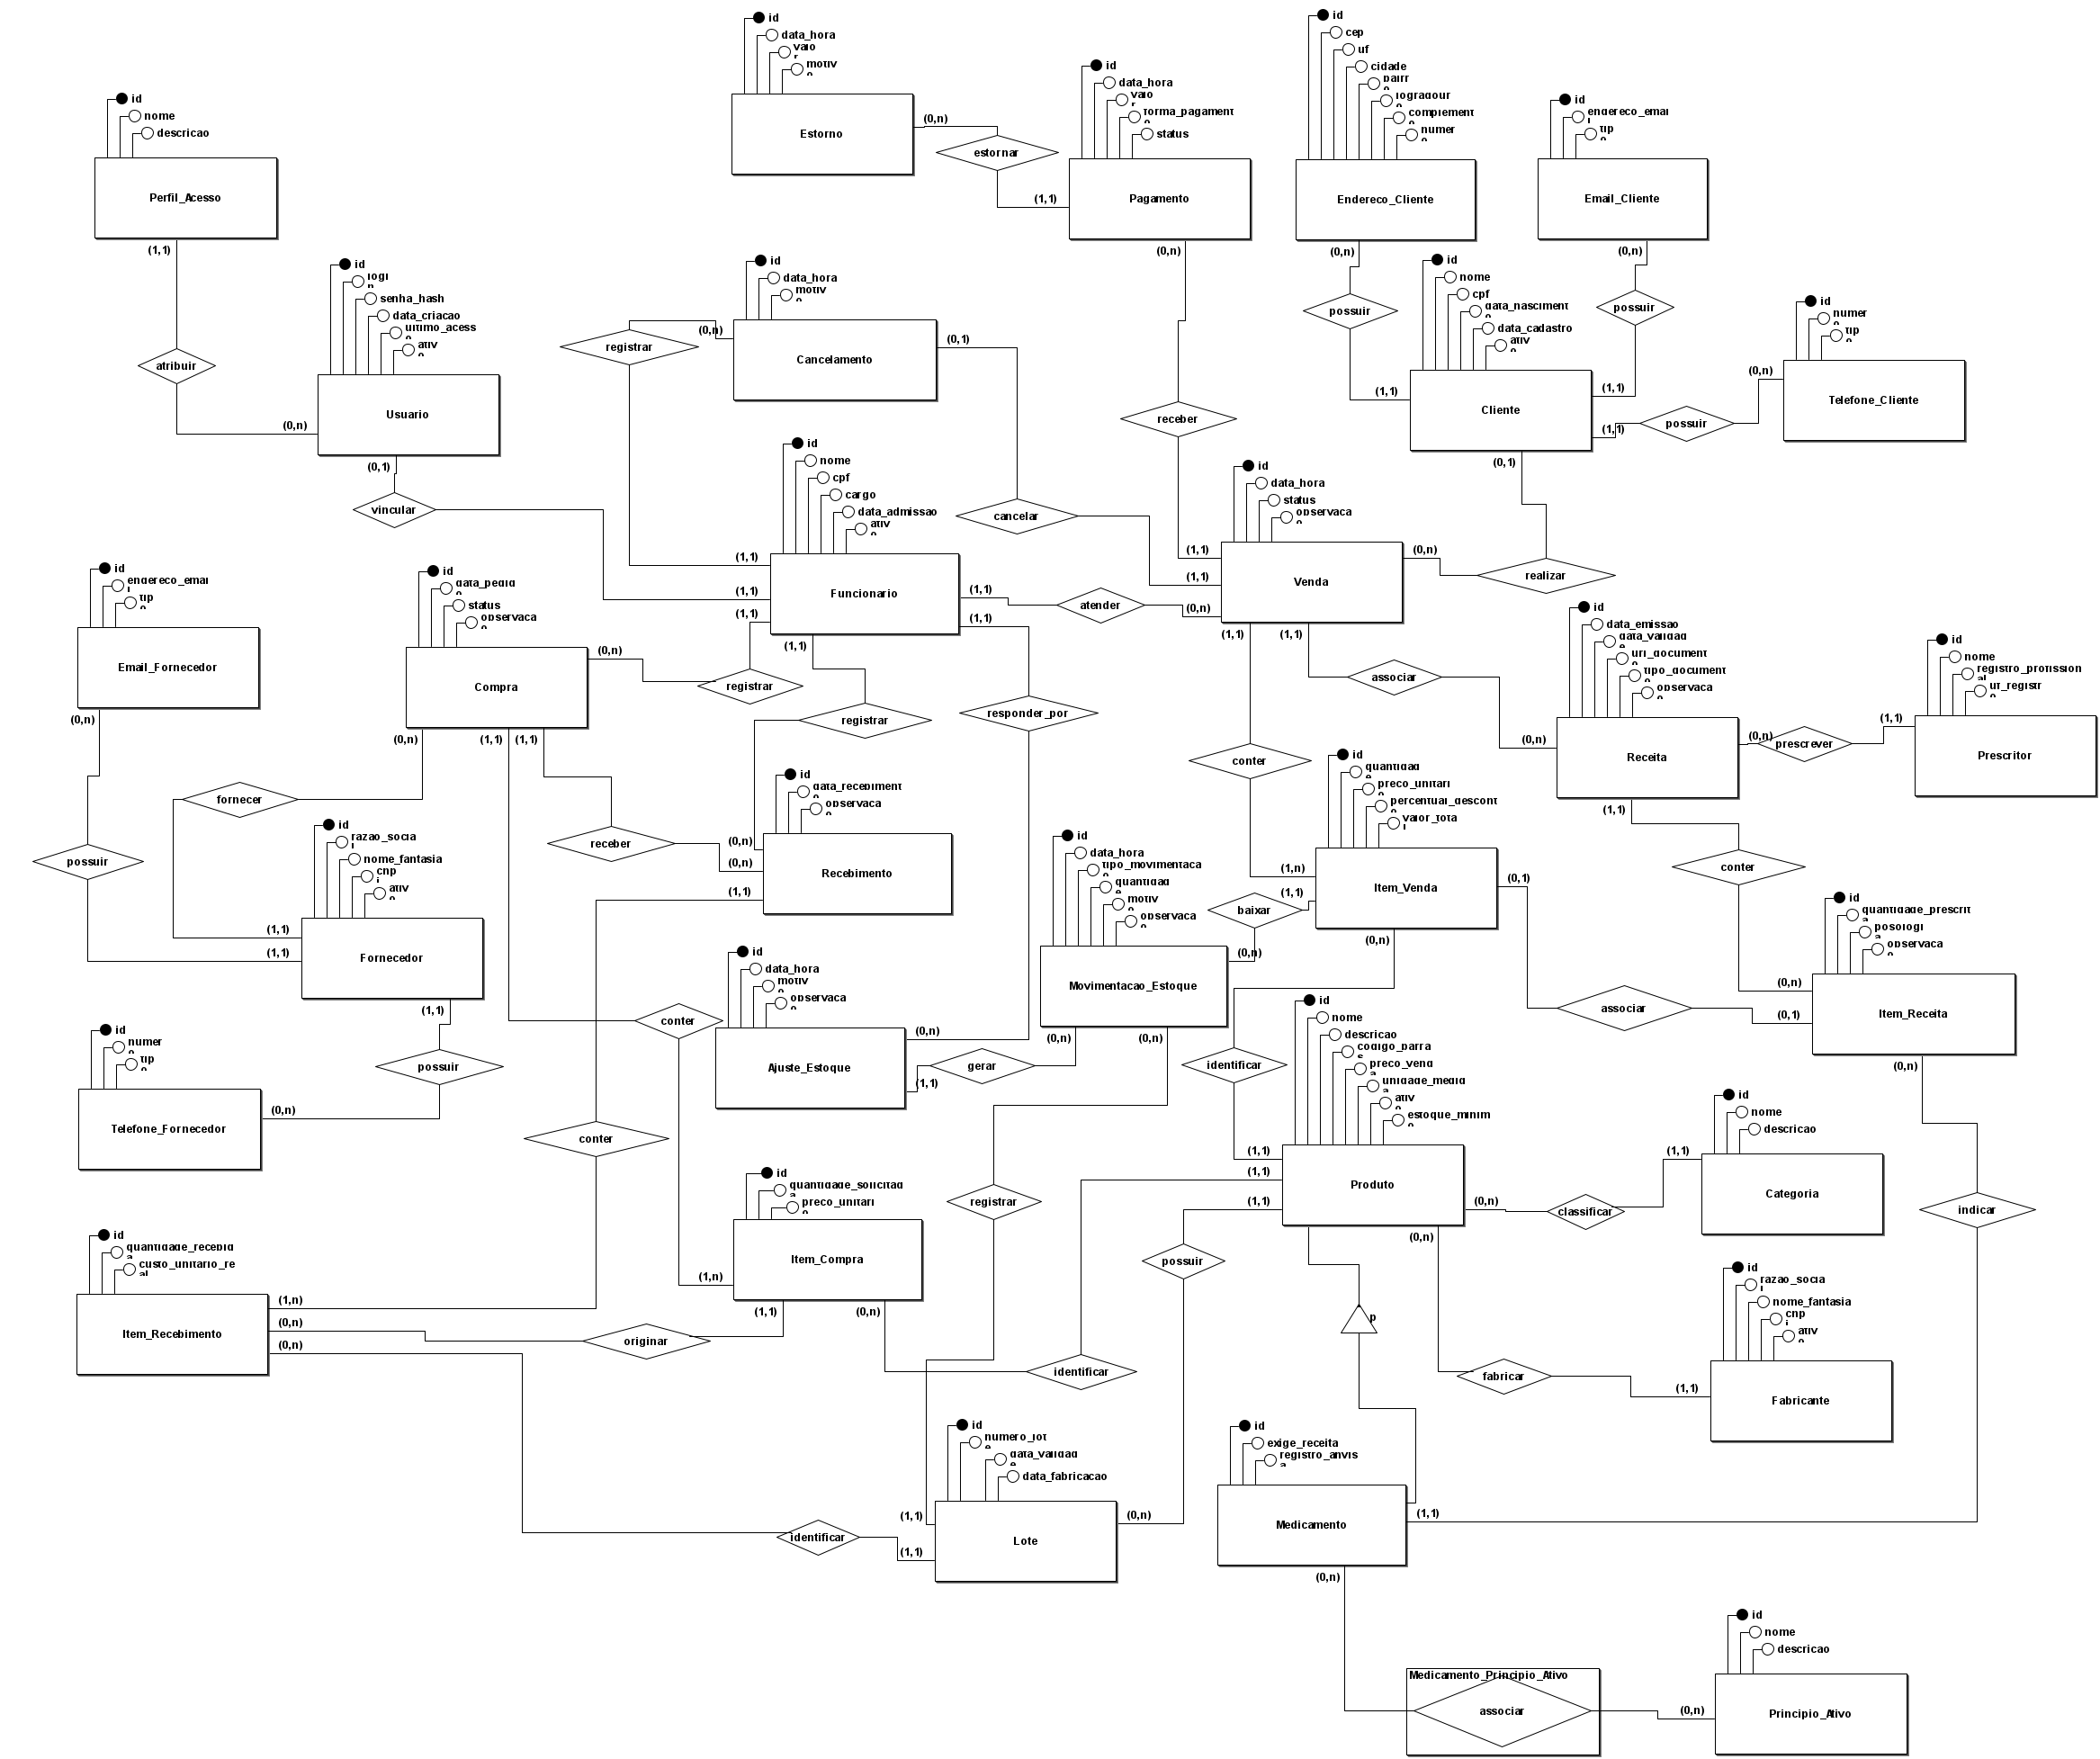
\includegraphics[width=0.96\linewidth,height=0.78\textheight,keepaspectratio]{../Drogaria_DER_Final.png}
\par\smallskip
\small\textbf{Fonte:} Elaborado pelos autores (2026).
\end{figure}
\end{landscape}

\clearpage
\begin{landscape}
\thispagestyle{fancy}
\begin{figure}[p]
\centering
\captionsetup{font=small,labelfont=bf,justification=centering}
\caption{Modelo logico relacional}
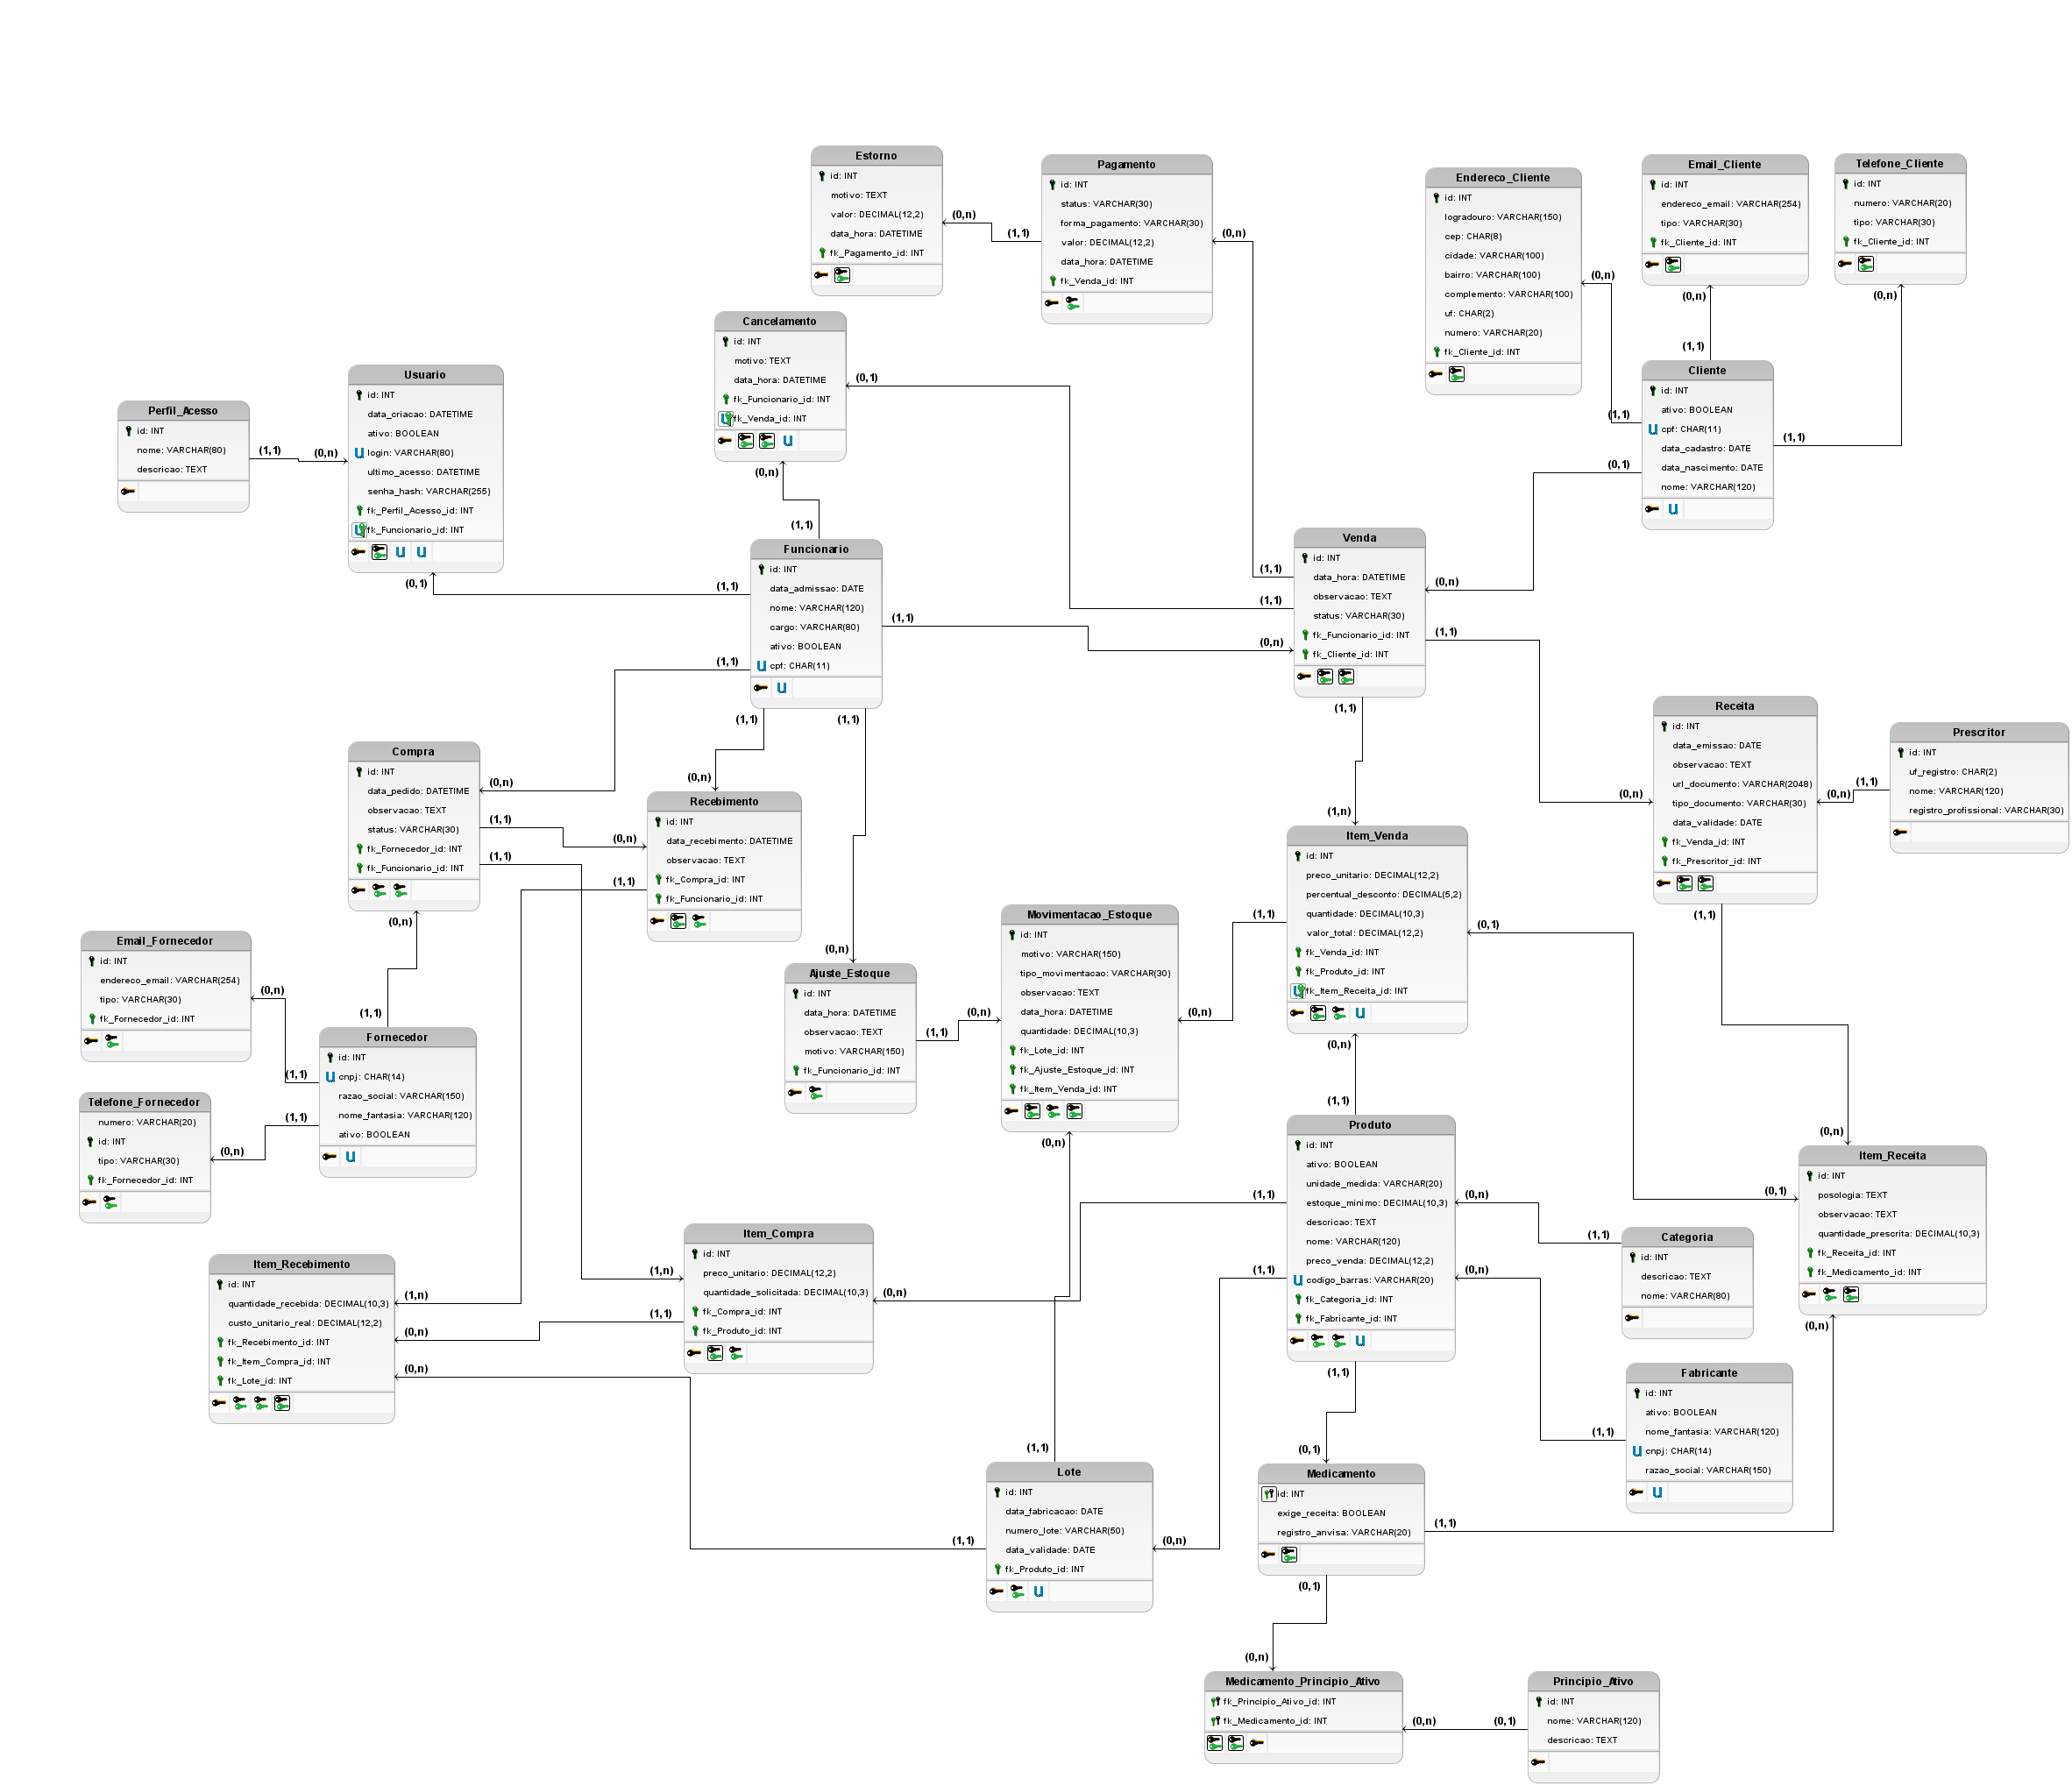
\includegraphics[width=0.96\linewidth,height=0.78\textheight,keepaspectratio]{../Drogaria_Logico.png}
\par\smallskip
\small\textbf{Fonte:} Elaborado pelos autores (2026).
\end{figure}
\end{landscape}

\clearpage
\section{Dicionario de dados}
O dicionario de dados descreve os atributos do modelo logico, seus tipos adotados para MySQL, suas finalidades e as chaves existentes ou definidas para implementacao. Os marcadores apresentados na ultima coluna sao: PK (chave primaria), FK (chave estrangeira) e UNIQUE (valor unico). O DDL detalha as restricoes fisicas; o roteiro testa os cenarios indicados na Secao~\ref{sec:implementacao-validacao}, sem cobrir todas as regras de negocio descritas neste documento.

\begingroup
\small
\singlespacing
\setlength{\tabcolsep}{3pt}
\renewcommand{\arraystretch}{1.15}
\begin{longtable}{@{}|L{2.7cm}|L{2.2cm}|L{8.0cm}|L{2.2cm}|@{}}
\caption{Dicionario de dados do sistema}\\
\hline
\textbf{Atributo} & \textbf{Tipo MySQL} & \textbf{Descricao} & \textbf{Chaves}\\
\hline
\endfirsthead
\caption[]{Dicionario de dados do sistema (continuacao)}\\
\hline
\textbf{Atributo} & \textbf{Tipo MySQL} & \textbf{Descricao} & \textbf{Chaves}\\
\hline
\endhead
\hline
\multicolumn{4}{|r|}{Continua na proxima pagina.}\\
\endfoot
\hline
\endlastfoot

\dictgroup{Produto}
\dictrow{id}{INT}{Identificador do produto.}{PK}
\dictrow{ativo}{BOOLEAN}{Indica se o produto esta ativo para novas operacoes.}{--}
\dictrow{unidade_medida}{VARCHAR(20)}{Unidade usada para expressar a quantidade do produto.}{--}
\dictrow{estoque_minimo}{DECIMAL(10,3)}{Quantidade minima definida para apoiar o acompanhamento do estoque.}{--}
\dictrow{descricao}{TEXT}{Descricao complementar do produto.}{--}
\dictrow{nome}{VARCHAR(120)}{Nome de cadastro do produto.}{--}
\dictrow{preco_venda}{DECIMAL(12,2)}{Preco atual de venda cadastrado para o produto.}{--}
\dictrow{codigo_barras}{VARCHAR(20)}{Codigo de barras do produto, unico quando informado.}{UNIQUE}
\dictrow{fk_Categoria_id}{INT}{Categoria principal associada ao produto.}{FK}
\dictrow{fk_Fabricante_id}{INT}{Fabricante associado ao produto.}{FK}

\dictgroup{Categoria}
\dictrow{id}{INT}{Identificador da categoria.}{PK}
\dictrow{descricao}{TEXT}{Descricao da categoria.}{--}
\dictrow{nome}{VARCHAR(80)}{Nome da categoria.}{--}

\dictgroup{Fabricante}
\dictrow{id}{INT}{Identificador do fabricante.}{PK}
\dictrow{ativo}{BOOLEAN}{Indica se o fabricante esta ativo para novos cadastros ou operacoes.}{--}
\dictrow{nome_fantasia}{VARCHAR(120)}{Nome fantasia do fabricante.}{--}
\dictrow{cnpj}{CHAR(14)}{CNPJ unico do fabricante, armazenado sem mascara.}{UNIQUE}
\dictrow{razao_social}{VARCHAR(150)}{Razao social do fabricante.}{--}

\dictgroup{Medicamento}
\dictrow{id}{INT}{Identificador do medicamento, compartilhado com o produto correspondente.}{PK/FK}
\dictrow{exige_receita}{BOOLEAN}{Indica se a venda do medicamento exige receita conforme o cadastro.}{--}
\dictrow{registro_anvisa}{VARCHAR(20)}{Numero ou codigo de registro do medicamento na Anvisa, quando aplicavel.}{--}

\dictgroup{Principio\_Ativo}
\dictrow{id}{INT}{Identificador do principio ativo.}{PK}
\dictrow{nome}{VARCHAR(120)}{Nome do principio ativo.}{--}
\dictrow{descricao}{TEXT}{Descricao complementar do principio ativo.}{--}

\dictgroup{Lote}
\dictrow{id}{INT}{Identificador do lote.}{PK}
\dictrow{data_fabricacao}{DATE}{Data de fabricacao do lote, quando informada.}{--}
\dictrow{numero_lote}{VARCHAR(50)}{Numero do lote; unico em conjunto com o produto.}{UNIQUE/\allowbreak composta}
\dictrow{data_validade}{DATE}{Data de validade do lote, quando aplicavel.}{--}
\dictrow{fk_Produto_id}{INT}{Produto ao qual o lote pertence.}{FK}

\dictgroup{Movimentacao\_Estoque}
\dictrow{id}{INT}{Identificador da movimentacao de estoque.}{PK}
\dictrow{motivo}{VARCHAR(150)}{Motivo textual da movimentacao, quando informado.}{--}
\dictrow{tipo_movimentacao}{VARCHAR(30)}{Classificacao da movimentacao, como entrada, saida ou ajuste.}{--}
\dictrow{observacao}{TEXT}{Observacoes adicionais sobre a movimentacao.}{--}
\dictrow{data_hora}{DATETIME}{Data e hora em que a movimentacao foi registrada.}{--}
\dictrow{quantidade}{DECIMAL(10,3)}{Quantidade movimentada no lote.}{--}
\dictrow{fk_Lote_id}{INT}{Lote de estoque afetado pela movimentacao.}{FK}
\dictrow{fk_Ajuste_Estoque_id}{INT}{Ajuste de estoque relacionado, quando a movimentacao decorrer de ajuste.}{FK}
\dictrow{fk_Item_Venda_id}{INT}{Item de venda relacionado, quando a movimentacao decorrer de venda.}{FK}

\dictgroup{Ajuste\_Estoque}
\dictrow{id}{INT}{Identificador do ajuste de estoque.}{PK}
\dictrow{data_hora}{DATETIME}{Data e hora em que o ajuste foi registrado.}{--}
\dictrow{observacao}{TEXT}{Observacoes complementares sobre o ajuste.}{--}
\dictrow{motivo}{VARCHAR(150)}{Motivo do ajuste de estoque.}{--}
\dictrow{fk_Funcionario_id}{INT}{Funcionario responsavel pelo ajuste.}{FK}

\dictgroup{Fornecedor}
\dictrow{id}{INT}{Identificador do fornecedor.}{PK}
\dictrow{cnpj}{CHAR(14)}{CNPJ unico do fornecedor, armazenado sem mascara.}{UNIQUE}
\dictrow{razao_social}{VARCHAR(150)}{Razao social do fornecedor.}{--}
\dictrow{nome_fantasia}{VARCHAR(120)}{Nome fantasia do fornecedor.}{--}
\dictrow{ativo}{BOOLEAN}{Indica se o fornecedor esta ativo para novas operacoes.}{--}

\dictgroup{Telefone\_Fornecedor}
\dictrow{numero}{VARCHAR(20)}{Numero de telefone do fornecedor.}{--}
\dictrow{id}{INT}{Identificador do registro de telefone.}{PK}
\dictrow{tipo}{VARCHAR(30)}{Tipo ou finalidade do telefone, quando informado.}{--}
\dictrow{fk_Fornecedor_id}{INT}{Fornecedor ao qual o telefone pertence.}{FK}

\dictgroup{Email\_Fornecedor}
\dictrow{id}{INT}{Identificador do registro de e-mail.}{PK}
\dictrow{endereco_email}{VARCHAR(254)}{Endereco de e-mail do fornecedor.}{--}
\dictrow{tipo}{VARCHAR(30)}{Tipo ou finalidade do e-mail, quando informado.}{--}
\dictrow{fk_Fornecedor_id}{INT}{Fornecedor ao qual o e-mail pertence.}{FK}

\dictgroup{Compra}
\dictrow{id}{INT}{Identificador do pedido de compra.}{PK}
\dictrow{data_pedido}{DATETIME}{Data e hora de registro do pedido.}{--}
\dictrow{observacao}{TEXT}{Observacoes sobre o pedido de compra.}{--}
\dictrow{status}{VARCHAR(30)}{Situacao do pedido, armazenada e atualizada quando ha recebimentos.}{--}
\dictrow{fk_Fornecedor_id}{INT}{Fornecedor ao qual o pedido foi feito.}{FK}
\dictrow{fk_Funcionario_id}{INT}{Funcionario responsavel pelo pedido.}{FK}

\dictgroup{Item\_Compra}
\dictrow{id}{INT}{Identificador do item do pedido de compra.}{PK}
\dictrow{preco_unitario}{DECIMAL(12,2)}{Preco unitario negociado para o item no pedido.}{--}
\dictrow{quantidade_solicitada}{DECIMAL(10,3)}{Quantidade solicitada do produto.}{--}
\dictrow{fk_Compra_id}{INT}{Pedido de compra ao qual o item pertence.}{FK}
\dictrow{fk_Produto_id}{INT}{Produto solicitado no item de compra.}{FK}

\dictgroup{Recebimento}
\dictrow{id}{INT}{Identificador do recebimento.}{PK}
\dictrow{data_recebimento}{DATETIME}{Data e hora em que o recebimento foi registrado.}{--}
\dictrow{observacao}{TEXT}{Observacoes complementares sobre o recebimento.}{--}
\dictrow{fk_Compra_id}{INT}{Pedido de compra relacionado ao recebimento.}{FK}
\dictrow{fk_Funcionario_id}{INT}{Funcionario responsavel pelo registro do recebimento.}{FK}

\dictgroup{Item\_Recebimento}
\dictrow{id}{INT}{Identificador do item recebido.}{PK}
\dictrow{quantidade_recebida}{DECIMAL(10,3)}{Quantidade efetivamente recebida do item.}{--}
\dictrow{custo_unitario_real}{DECIMAL(12,2)}{Custo unitario efetivo desta entrega; fonte do custo por recebimento.}{--}
\dictrow{fk_Recebimento_id}{INT}{Recebimento ao qual o item pertence.}{FK}
\dictrow{fk_Item_Compra_id}{INT}{Item do pedido de compra atendido pelo recebimento.}{FK}
\dictrow{fk_Lote_id}{INT}{Lote associado aos produtos recebidos, quando aplicavel.}{FK}

\dictgroup{Venda}
\dictrow{id}{INT}{Identificador da venda.}{PK}
\dictrow{data_hora}{DATETIME}{Data e hora em que a venda foi registrada.}{--}
\dictrow{observacao}{TEXT}{Observacoes complementares sobre a venda.}{--}
\dictrow{status}{VARCHAR(30)}{Situacao operacional da venda.}{--}
\dictrow{fk_Funcionario_id}{INT}{Funcionario responsavel pela venda.}{FK}
\dictrow{fk_Cliente_id}{INT}{Cliente associado a venda, quando informado.}{FK}

\dictgroup{Item\_Venda}
\dictrow{id}{INT}{Identificador do item de venda.}{PK}
\dictrow{preco_unitario}{DECIMAL(12,2)}{Preco unitario praticado no momento da venda.}{--}
\dictrow{percentual_desconto}{DECIMAL(5,2)}{Percentual de desconto aplicado ao item.}{--}
\dictrow{quantidade}{DECIMAL(10,3)}{Quantidade vendida do produto.}{--}
\dictrow{valor_total}{DECIMAL(12,2)}{Valor final do item, mantido no modelo e atualizado conforme quantidade, preco unitario e desconto.}{--}
\dictrow{fk_Venda_id}{INT}{Venda a que o item pertence.}{FK}
\dictrow{fk_Produto_id}{INT}{Produto vendido.}{FK}
\dictrow{fk_Item_Receita_id}{INT}{Item de receita associado a venda, quando houver.}{FK/\allowbreak UNIQUE}

\dictgroup{Pagamento}
\dictrow{id}{INT}{Identificador do pagamento.}{PK}
\dictrow{status}{VARCHAR(30)}{Situacao do pagamento.}{--}
\dictrow{forma_pagamento}{VARCHAR(30)}{Modalidade utilizada no pagamento.}{--}
\dictrow{valor}{DECIMAL(12,2)}{Valor registrado para o pagamento.}{--}
\dictrow{data_hora}{DATETIME}{Data e hora em que o pagamento foi registrado.}{--}
\dictrow{fk_Venda_id}{INT}{Venda a que o pagamento esta associado.}{FK}

\dictgroup{Estorno}
\dictrow{id}{INT}{Identificador do estorno.}{PK}
\dictrow{motivo}{TEXT}{Motivo do estorno.}{--}
\dictrow{valor}{DECIMAL(12,2)}{Valor estornado do pagamento.}{--}
\dictrow{data_hora}{DATETIME}{Data e hora em que o estorno foi registrado.}{--}
\dictrow{fk_Pagamento_id}{INT}{Pagamento ao qual o estorno se refere.}{FK}

\dictgroup{Cancelamento}
\dictrow{id}{INT}{Identificador do cancelamento.}{PK}
\dictrow{motivo}{TEXT}{Motivo informado para o cancelamento da venda.}{--}
\dictrow{data_hora}{DATETIME}{Data e hora em que o cancelamento foi registrado.}{--}
\dictrow{fk_Funcionario_id}{INT}{Funcionario responsavel pelo cancelamento.}{FK}
\dictrow{fk_Venda_id}{INT}{Venda cancelada; o modelo marca a referencia como unica.}{FK/\allowbreak UNIQUE}

\dictgroup{Cliente}
\dictrow{id}{INT}{Identificador do cliente.}{PK}
\dictrow{ativo}{BOOLEAN}{Indica se o cadastro do cliente esta ativo.}{--}
\dictrow{cpf}{CHAR(11)}{CPF unico quando informado, armazenado sem mascara.}{UNIQUE}
\dictrow{data_cadastro}{DATE}{Data em que o cliente foi cadastrado.}{--}
\dictrow{data_nascimento}{DATE}{Data de nascimento do cliente.}{--}
\dictrow{nome}{VARCHAR(120)}{Nome do cliente.}{--}

\dictgroup{Telefone\_Cliente}
\dictrow{id}{INT}{Identificador do registro de telefone.}{PK}
\dictrow{numero}{VARCHAR(20)}{Numero de telefone do cliente.}{--}
\dictrow{tipo}{VARCHAR(30)}{Tipo ou finalidade do telefone, quando informado.}{--}
\dictrow{fk_Cliente_id}{INT}{Cliente ao qual o telefone pertence.}{FK}

\dictgroup{Email\_Cliente}
\dictrow{endereco_email}{VARCHAR(254)}{Endereco de e-mail do cliente.}{--}
\dictrow{id}{INT}{Identificador do registro de e-mail.}{PK}
\dictrow{tipo}{VARCHAR(30)}{Tipo ou finalidade do e-mail, quando informado.}{--}
\dictrow{fk_Cliente_id}{INT}{Cliente ao qual o e-mail pertence.}{FK}

\dictgroup{Endereco\_Cliente}
\dictrow{logradouro}{VARCHAR(150)}{Logradouro do endereco do cliente.}{--}
\dictrow{id}{INT}{Identificador do endereco.}{PK}
\dictrow{cep}{CHAR(8)}{CEP do endereco, armazenado sem mascara.}{--}
\dictrow{cidade}{VARCHAR(100)}{Cidade do endereco.}{--}
\dictrow{bairro}{VARCHAR(100)}{Bairro do endereco.}{--}
\dictrow{complemento}{VARCHAR(100)}{Complemento do endereco, quando informado.}{--}
\dictrow{uf}{CHAR(2)}{Sigla da unidade federativa.}{--}
\dictrow{numero}{VARCHAR(20)}{Numero ou identificacao do imovel, incluindo valores como S/N.}{--}
\dictrow{fk_Cliente_id}{INT}{Cliente ao qual o endereco pertence.}{FK}

\dictgroup{Funcionario}
\dictrow{id}{INT}{Identificador do funcionario.}{PK}
\dictrow{data_admissao}{DATE}{Data de admissao do funcionario.}{--}
\dictrow{nome}{VARCHAR(120)}{Nome do funcionario.}{--}
\dictrow{cargo}{VARCHAR(80)}{Cargo ou funcao exercida pelo funcionario.}{--}
\dictrow{ativo}{BOOLEAN}{Indica se o funcionario esta ativo.}{--}
\dictrow{cpf}{CHAR(11)}{CPF unico do funcionario, armazenado sem mascara.}{UNIQUE}

\dictgroup{Usuario}
\dictrow{id}{INT}{Identificador do usuario do sistema.}{PK}
\dictrow{data_criacao}{DATETIME}{Data e hora de criacao da conta.}{--}
\dictrow{ativo}{BOOLEAN}{Indica se a conta de usuario esta ativa.}{--}
\dictrow{login}{VARCHAR(80)}{Identificador unico de login utilizado pelo usuario.}{UNIQUE}
\dictrow{ultimo_acesso}{DATETIME}{Data e hora do ultimo acesso registrado.}{--}
\dictrow{senha_hash}{VARCHAR(255)}{Hash da senha armazenado para autenticacao; nao representa a senha em texto puro.}{--}
\dictrow{fk_Perfil_Acesso_id}{INT}{Perfil de acesso associado ao usuario.}{FK}
\dictrow{fk_Funcionario_id}{INT}{Funcionario associado a conta; o modelo marca a referencia como unica.}{FK/\allowbreak UNIQUE}

\dictgroup{Perfil\_Acesso}
\dictrow{id}{INT}{Identificador do perfil de acesso.}{PK}
\dictrow{nome}{VARCHAR(80)}{Nome do perfil de acesso.}{--}
\dictrow{descricao}{TEXT}{Descricao das permissoes ou finalidade do perfil.}{--}

\dictgroup{Receita}
\dictrow{id}{INT}{Identificador da receita.}{PK}
\dictrow{data_emissao}{DATE}{Data de emissao da receita.}{--}
\dictrow{observacao}{TEXT}{Observacoes complementares sobre a receita.}{--}
\dictrow{url_documento}{VARCHAR(2048)}{URL ou referencia protegida do documento da receita.}{--}
\dictrow{tipo_documento}{VARCHAR(30)}{Classificacao do documento de receita.}{--}
\dictrow{data_validade}{DATE}{Data de validade da receita, quando informada.}{--}
\dictrow{fk_Venda_id}{INT}{Venda a que a receita esta associada.}{FK}
\dictrow{fk_Prescritor_id}{INT}{Prescritor responsavel pela receita.}{FK}

\dictgroup{Item\_Receita}
\dictrow{id}{INT}{Identificador do item de receita.}{PK}
\dictrow{posologia}{TEXT}{Orientacao de uso prescrita para o medicamento.}{--}
\dictrow{observacao}{TEXT}{Observacoes complementares do item de receita.}{--}
\dictrow{quantidade_prescrita}{DECIMAL(10,3)}{Quantidade do medicamento indicada na receita.}{--}
\dictrow{fk_Receita_id}{INT}{Receita a que o item pertence.}{FK}
\dictrow{fk_Medicamento_id}{INT}{Medicamento prescrito no item.}{FK}

\dictgroup{Prescritor}
\dictrow{id}{INT}{Identificador do prescritor.}{PK}
\dictrow{uf_registro}{CHAR(2)}{Sigla da unidade federativa do registro profissional.}{--}
\dictrow{nome}{VARCHAR(120)}{Nome do prescritor.}{--}
\dictrow{registro_profissional}{VARCHAR(30)}{Numero do registro profissional do prescritor.}{--}

\dictgroup{Medicamento\_Principio\_Ativo}
\dictrow{fk_Principio_Ativo_id}{INT}{Principio ativo associado ao medicamento; participa da chave composta.}{PK/FK}
\dictrow{fk_Medicamento_id}{INT}{Medicamento associado ao principio ativo; participa da chave composta.}{PK/FK}

\end{longtable}
\endgroup

\section{Análise de normalização}
\subsection{Escopo e dependências funcionais consideradas}
Foram avaliadas as 31 relacoes do modelo logico. O banco foi implementado e exercitado com dados sinteticos temporarios, mas a analise de normalizacao permanece estrutural: considera as chaves candidatas e as dependencias funcionais decorrentes das regras do esquema, e nao depende de dados de producao. A fundamentacao relacional segue o modelo de Codd (1970).

O Quadro~\ref{tab:chaves-normalizacao} resume as chaves consideradas e as unicidades definidas. As regras RB29 e RB32 determinam a unicidade do codigo de barras informado e a identificacao de lote pela combinacao de produto e numero do lote. O DDL implementa essas restricoes, assim como as unicidades de CPF, CNPJ, login e das referencias que representam relacoes 1:1.

\begingroup
\small
\singlespacing
\setlength{\tabcolsep}{3pt}
\renewcommand{\arraystretch}{1.12}
\begin{longtable}{|L{3.5cm}|L{6.0cm}|L{5.2cm}|}
\caption{Chaves consideradas na analise de normalizacao}\label{tab:chaves-normalizacao}\\
\hline
\textbf{Relacao} & \textbf{Chave primaria e candidatas} & \textbf{Observacao}\\
\hline
\endfirsthead
\caption[]{Chaves consideradas na analise de normalizacao (continuacao)}\\
\hline
\textbf{Relacao} & \textbf{Chave primaria e candidatas} & \textbf{Observacao}\\
\hline
\endhead
\hline
\multicolumn{3}{|r|}{Continua na proxima pagina.}\\
\endfoot
\hline
\endlastfoot
Produto & \texttt{id}; \url{codigo_barras} & Codigo de barras unico quando informado (RB29); implementado no DDL.\\\hline
Categoria & \texttt{id} & --\\\hline
Fabricante & \texttt{id}; \texttt{cnpj} & CNPJ único.\\\hline
Medicamento & \texttt{id} & Chave primaria compartilhada com a chave estrangeira para Produto.\\\hline
\url{Principio_Ativo} & \texttt{id} & --\\\hline
Lote & \texttt{id}; (\url{fk_Produto_id}, \url{numero_lote}) & Chave alternativa composta da RB32; implementada como UNIQUE no DDL.\\\hline
\url{Movimentacao_Estoque} & \texttt{id} & --\\\hline
\url{Ajuste_Estoque} & \texttt{id} & --\\\hline
Fornecedor & \texttt{id}; \texttt{cnpj} & CNPJ único.\\\hline
\url{Telefone_Fornecedor} & \texttt{id} & --\\\hline
\url{Email_Fornecedor} & \texttt{id} & --\\\hline
Compra & \texttt{id} & --\\\hline
\url{Item_Compra} & \texttt{id} & --\\\hline
Recebimento & \texttt{id} & --\\\hline
\url{Item_Recebimento} & \texttt{id} & --\\\hline
Venda & \texttt{id} & --\\\hline
\url{Item_Venda} & \texttt{id}; \url{fk_Item_Receita_id} & A referencia a item de receita e unica quando informada.\\\hline
Pagamento & \texttt{id} & --\\\hline
Estorno & \texttt{id} & --\\\hline
Cancelamento & \texttt{id}; \texttt{fk\_Venda\_id} & Uma venda pode ter no maximo um cancelamento.\\\hline
Cliente & \texttt{id}; \texttt{cpf} & CPF único quando informado.\\\hline
\url{Telefone_Cliente} & \texttt{id} & --\\\hline
\url{Email_Cliente} & \texttt{id} & --\\\hline
\url{Endereco_Cliente} & \texttt{id} & --\\\hline
Funcionario & \texttt{id}; \texttt{cpf} & CPF único.\\\hline
Usuario & \texttt{id}; \texttt{fk\_Funcionario\_id}; \texttt{login} & Funcionário associado e login únicos.\\\hline
\url{Perfil_Acesso} & \texttt{id} & --\\\hline
Receita & \texttt{id} & --\\\hline
\url{Item_Receita} & \texttt{id} & --\\\hline
Prescritor & \texttt{id} & A unicidade do registro profissional não foi definida.\\\hline
\url{Medicamento_Principio_Ativo} & (\url{fk_Medicamento_id}, \url{fk_Principio_Ativo_id}) & Chave primaria composta; nao ha atributos nao-chave.\\\hline
\end{longtable}
\endgroup

\subsection{Primeira Forma Normal (1FN)}
As relações atendem estruturalmente à 1FN: cada campo representa um valor por registro, sem listas de telefones, e-mails, endereços ou princípios ativos armazenadas dentro de uma única coluna. Os contatos de clientes e fornecedores foram separados em relações próprias, e a associação entre medicamentos e princípios ativos foi representada por uma relação associativa. Campos textuais, como observações e descrições, são tratados como valores atômicos do ponto de vista relacional; seu conteúdo livre não representa uma lista estruturada de atributos.

\subsection{Segunda Forma Normal (2FN)}
As relacoes cuja chave primaria e simples atendem a 2FN, pois nao existe dependencia parcial em uma chave de um unico atributo. A unica chave primaria composta e a de \texttt{Medicamento\_Principio\_Ativo}; essa relacao contem somente as duas chaves estrangeiras que compoem a propria chave, sem atributo nao-chave sujeito a dependencia parcial. A chave alternativa composta de \texttt{Lote}, definida por produto e numero do lote, esta implementada como restricao unica composta no DDL.

\subsection{Terceira Forma Normal (3FN)}
Considerando as dependências funcionais identificadas, não há atributo não-chave que determine outro atributo não-chave dentro da mesma relação. Dados de categorias e fabricantes ficam em suas próprias relações, dados de fornecedores não são repetidos em compras, dados de perfil não são copiados para usuários e os contatos múltiplos foram decompostos em relações separadas. Assim, não foram identificadas dependências transitivas que exijam nova decomposição para atingir a 3FN.

\subsection{Forma Normal de Boyce-Codd (BCNF)}
Pelas dependencias funcionais identificadas, os determinantes nao triviais sao chaves candidatas: as chaves primarias simples, as referencias unicas de \texttt{Usuario}, \texttt{Cancelamento} e \texttt{Item\_Venda}, as unicidades definidas para CPF, CNPJ e login, o codigo de barras quando preenchido e a identificacao composta de lote. Sob esse conjunto de dependencias, as relacoes atendem a BCNF. As unicidades consideradas estao implementadas no DDL; a conclusao continua condicionada a que as dependencias funcionais e as regras de negocio identificadas sejam completas.

\subsection{Decisoes refletidas no modelo fisico}
As decisoes abaixo foram incorporadas ao DDL ou permanecem sob responsabilidade da aplicacao cliente:
\begin{itemize}
\item \texttt{Item\_Venda.valor\_total} permanece armazenado. A aplicacao deve recalcula-lo a partir da quantidade, preco unitario e desconto; o DDL atual nao confere essa formula entre colunas.
\item O custo real e registrado em \texttt{Item\_Recebimento.custo\_unitario\_real}; \texttt{Lote.custo\_unitario} foi removido do modelo.
\item CPF de Cliente e Funcionario, CNPJ de Fornecedor e Fabricante e login de Usuario sao unicos no DDL. O registro profissional do prescritor permanece sem unicidade porque o modelo nao identifica o conselho ou a profissao.
\item \texttt{Compra.status} e armazenado e recalculado pela procedure e pelos triggers do DDL quando itens de recebimento sao inseridos, alterados ou excluidos.
\item Triggers do DDL validam a coerencia entre compra, recebimento e lote, e entre item de venda e item de receita/produto.
\item O DDL exige quantidade de movimentacao positiva e limita o tipo a ENTRADA, SAIDA, AJUSTE\_ENTRADA ou AJUSTE\_SAIDA. Essas restricoes nao impedem, por si, que o saldo agregado fique negativo.
\end{itemize}

\section{Implementacao fisica e validacao}
\label{sec:implementacao-validacao}

\subsection{Modelo fisico}
O modelo fisico foi implementado para MySQL 8.0 no arquivo \texttt{Drogaria\_Fisico.sql}. O script cria 31 tabelas, uma view de saldo de estoque, uma procedure para recalcular a situacao de compras e sete triggers. O DDL define chaves primarias e estrangeiras, unicidades e restricoes \texttt{CHECK}; os triggers validam a coerencia entre compra, recebimento e lote, atualizam o status de compras e validam a associacao entre venda e receita. O comportamento de \texttt{CHECK}, views e triggers segue a documentacao do MySQL 8.0 (Oracle, s. d.).

\subsection{Roteiro de testes}
O arquivo \texttt{Drogaria\_Testes.sql} prepara dados sinteticos e executa \texttt{INSERT}, \texttt{UPDATE} e \texttt{DELETE} nas 31 tabelas. As consultas de leitura verificam os fluxos de compra, venda e saldo de estoque; nao ha uma consulta individual para cada tabela. As alteracoes de dados ficam em uma transacao desfeita por \texttt{ROLLBACK}.

\subsection{Execucao e resultados}
O DDL e o roteiro foram executados em um banco MySQL 8.0.46 descartavel, sem erros de criacao. Os testes confirmaram os seguintes cenarios:

\begin{itemize}
\item O banco rejeita um item recebido associado a uma compra diferente daquela do recebimento.
\item O banco rejeita o recebimento de um lote pertencente a produto diferente daquele do item comprado.
\item O banco rejeita um item de venda cujo produto diverge do medicamento prescrito.
\item O banco rejeita a associacao de um item de receita pertencente a outra venda.
\item O status da compra passou de \texttt{PARCIALMENTE\_RECEBIDA} para \texttt{CONCLUIDA} apos recebimentos validos. A view retornou saldo \texttt{8,500} para as movimentacoes inseridas separadamente no roteiro; esse resultado nao demonstra que o recebimento criou uma movimentacao de entrada.
\end{itemize}

Os testes cobrem somente os cenarios descritos acima e nao comprovam todas as regras funcionais. A aplicacao cliente nao faz parte desta implementacao.

\subsection{Limites do DDL e responsabilidades da aplicacao}
O DDL atual nao implementa todos os requisitos funcionais como automacoes de banco. Os fluxos abaixo devem ser executados pela aplicacao cliente, em transacoes consistentes, ou receber implementacao complementar antes de serem considerados garantidos:

\begin{itemize}
\item O registro de um \texttt{Item\_Recebimento} nao cria automaticamente uma \texttt{Movimentacao\_Estoque}. A aplicacao deve registrar a entrada correspondente na mesma transacao. Conforme a decisao de modelagem, a entrada e rastreada pelo lote, sem chave estrangeira direta para o item recebido; por isso o DDL nao identifica qual recebimento especifico originou cada entrada.
\item A view calcula o saldo a partir das movimentacoes, mas o DDL nao bloqueia saldo negativo nem valida disponibilidade, validade do lote ou priorizacao FEFO antes de uma venda.
\item O DDL nao efetua a reversao de estoque no cancelamento nem vincula diretamente a movimentacao de retorno ao registro de cancelamento. A aplicacao deve aplicar a regra de devolucao aos lotes originais e preservar a rastreabilidade.
\item O DDL nao valida totais entre varias linhas de pagamento e estorno. Impedir pagamento acima do saldo, estorno acima do valor ainda disponivel e conclusao de venda sem pagamento integral depende do fluxo transacional da aplicacao.
\item A protecao da URL do documento de receita e a autorizacao por perfil tambem dependem da aplicacao e da configuracao de acesso; armazenar a referencia no banco nao protege o arquivo externo.
\end{itemize}

Essas regras permanecem no escopo funcional do sistema, mas nao foram demonstradas pelo DDL nem pelo roteiro atual. O registro de \texttt{valor\_total} em \texttt{Item\_Venda} tambem requer recalculo pela aplicacao, pois nao ha restricao ou trigger que compare o valor com quantidade, preco e desconto.
\section{Conclusao}
O documento consolida os requisitos, modelos conceitual e logico, dicionario de dados e analise de normalizacao, e descreve o DDL fisico e os testes executados. O esquema implementa as restricoes relacionais e os cenarios explicitamente descritos; regras que dependem de fluxos transacionais da aplicacao estao identificadas como pendentes de implementacao no cliente.
\clearpage
\section*{REFERÊNCIAS}
\addcontentsline{toc}{section}{REFERÊNCIAS}
\begingroup
\small
\singlespacing
\setlength{\parindent}{0pt}
\setlength{\parskip}{6pt}

ASSOCIAÇÃO BRASILEIRA DE NORMAS TÉCNICAS. \textbf{ABNT NBR 10520:2023}: informação e documentação: citações em documentos: apresentação. Rio de Janeiro: ABNT, 2023.

ASSOCIAÇÃO BRASILEIRA DE NORMAS TÉCNICAS. \textbf{ABNT NBR 14724:2024}: informação e documentação: trabalhos acadêmicos: apresentação. Rio de Janeiro: ABNT, 2024.

ASSOCIAÇÃO BRASILEIRA DE NORMAS TÉCNICAS. \textbf{ABNT NBR 6023:2025}: informação e documentação: referências: elaboração. Rio de Janeiro: ABNT, 2025.

CHEN, Peter Pin-Shan. The entity-relationship model: toward a unified view of data. \textit{ACM Transactions on Database Systems}, v. 1, n. 1, p. 9--36, 1976. DOI: \url{https://doi.org/10.1145/320434.320440}.

CODD, Edgar F. A relational model of data for large shared data banks. \textit{Communications of the ACM}, v. 13, n. 6, p. 377--387, 1970. DOI: \url{https://doi.org/10.1145/362384.362685}.

ORACLE. \textbf{MySQL 8.0 Reference Manual}. [S. l.]: Oracle, [s. d.]. Disponível em: \url{https://dev.mysql.com/doc/refman/8.0/en/}. Acesso em: 27 out. 2026.

\endgroup
\end{document}
